\documentclass[12pt,fleqn]{article}

\usepackage[utf8]{inputenc}
\usepackage[T2A]{fontenc}
\usepackage{amssymb,amsmath,mathrsfs,amsthm}
\usepackage[russian]{babel}
\usepackage[pdftex]{graphicx}
\usepackage{multirow}
\usepackage[footnotesize]{caption2}
\usepackage{indentfirst}
\usepackage[colorlinks,linkcolor=blue(ryb),citecolor=blue(ryb), unicode]{hyperref}

\usepackage{xcolor}
\usepackage{sectsty}

\definecolor{blue(ryb)}{rgb}{0.01, 0.28, 1.0}
%\usepackage[ruled,section]{algorithm}
%\usepackage[noend]{algorithmic}
%\usepackage[all]{xy}

% Параметры страницы
\textheight=24cm % высота текста
\textwidth=16cm % ширина текста
\oddsidemargin=0pt % отступ от левого края
\topmargin=-2.5cm % отступ от верхнего края
\parindent=24pt % абзацный отступ
\parskip=0pt % интервал между абзацам
\tolerance=2000 % терпимость к "жидким" строкам
\flushbottom % выравнивание высоты страниц
%\def\baselinestretch{1.5}
\setcounter{secnumdepth}{0}
\renewcommand{\baselinestretch}{1.1}

\newcommand{\norm}{\mathop{\rm norm}\limits}
\newcommand{\real}{\mathbb{R}}

\newcommand{\ex}{\mathbb{E}}
\newcommand{\diag}{\mathrm{diag}}
\newcommand{\intset}{\mathrm{int}}
\newcommand{\softmax}{\mathop{\rm softmax}\limits}
\newcommand{\lossfunc}{\mathcal{L}'}
\newcommand{\elbo}{\mathcal{L}}
\newcommand{\normal}[3]{\mathcal{N}(#1 | #2, #3)}
\newcommand{\dd}[2]{\frac{\partial#1}{\partial#2}}
\newcommand{\kl}[2]{\mathop{KL}(#1 \parallel #2)}
\newcommand{\nm}{\mathcal{N}}
\newcommand{\sle}{\; \Rightarrow \;}
\newcommand{\indpos}{\mathbf{I}_{d_k}^{+}[i, j]}
\newcommand{\indneg}{\mathbf{I}_{d_k}^{-}[i, j]}

\usepackage{pgfplots}

%my settings
\usepackage{titling}
\renewcommand\maketitlehooka{\null\mbox{}\vfill}
\renewcommand\maketitlehookd{\vfill\null}
\graphicspath{{../figures/}}
\usepackage{wrapfig}

\title{Отчет о проделанной работе в семестре}

\author{Тыцкий Владислав}
\date{Декабрь 2020 г.}
\begin{document}

\begin{center}
    \textbf{\Large{Московский государственный университет имени М.В. Ломоносова}} \\
		\vspace{4em}
		\textbf{\Large{Факультет вычислительной математики и кибернетики}} \\
		\vspace{4em}
		\textbf{\Large{Кафедра математических методов прогнозирования}} 
			\vspace{4em}
		
	\end{center}
	

	
	\vspace{12em}
	
	\begin{center}
        \textbf{\LARGE{ГРАФИК В ПАРАЛЛЕЛЬНЫХ ОСЯХ\linebreak \linebreak
         И ЕГО ПРИЛОЖЕНИЯ}}
	\end{center}
	
	\vspace{2em}
	
	\begin{center}
        \large{Семестровый отчет студента 3 курса\linebreak
         Тыцкого Владислава}
	\end{center}
	
	\vspace{6em}
	
	\begin{flushleft}
		
	\large{	Научный руководитель \linebreak
	к.ф.-м.н. доцент Майсурадзе А.И.}\\
		\vspace{1.5em}
	
	
	\end{flushleft}
	
	\vspace{\fill}
	
	\begin{center}
	\textbf{{\large Москва 2020}}
	\end{center}
	\thispagestyle{empty} 
\newpage
\section{Аннотация}
В данном отчете представлен обзор графика в параллельных осях(parallel coordinates)
и его модификаций, описание собственной библиотеки для построения данных графиков и
итоги работы над ней.

\section{Введение}
В анализе данных важной частью любого исследования является представление данных\footnote{
Часто будут использоваться синонимы выборка, датасет}
в наглядной для человека форме. 
Это необходимо не только для самого исследователя, но и для тех, кто читает исследование.

Для представления данных низкой размерности (до 3-ей) существует множество
вариантов визуализации. Однако далеко не все эти методы подходят для
высокоразмерных данных. Это является фундаментальной проблемой
представления информации на экране компьютера.
Её обходят по-разному: через представление координат (одной и более) как параметры и рисование нескольких
диаграмм для низкоразмерных данных, через рисование проекций на подпространства или через агрегирование
выборки. Но среди всех способов визуализации можно выделить так называемый график в
параллельных осях (parallel coordinates).

\newpage

\section{График в параллельных осях}

\begin{figure}[htb]
    \centering
    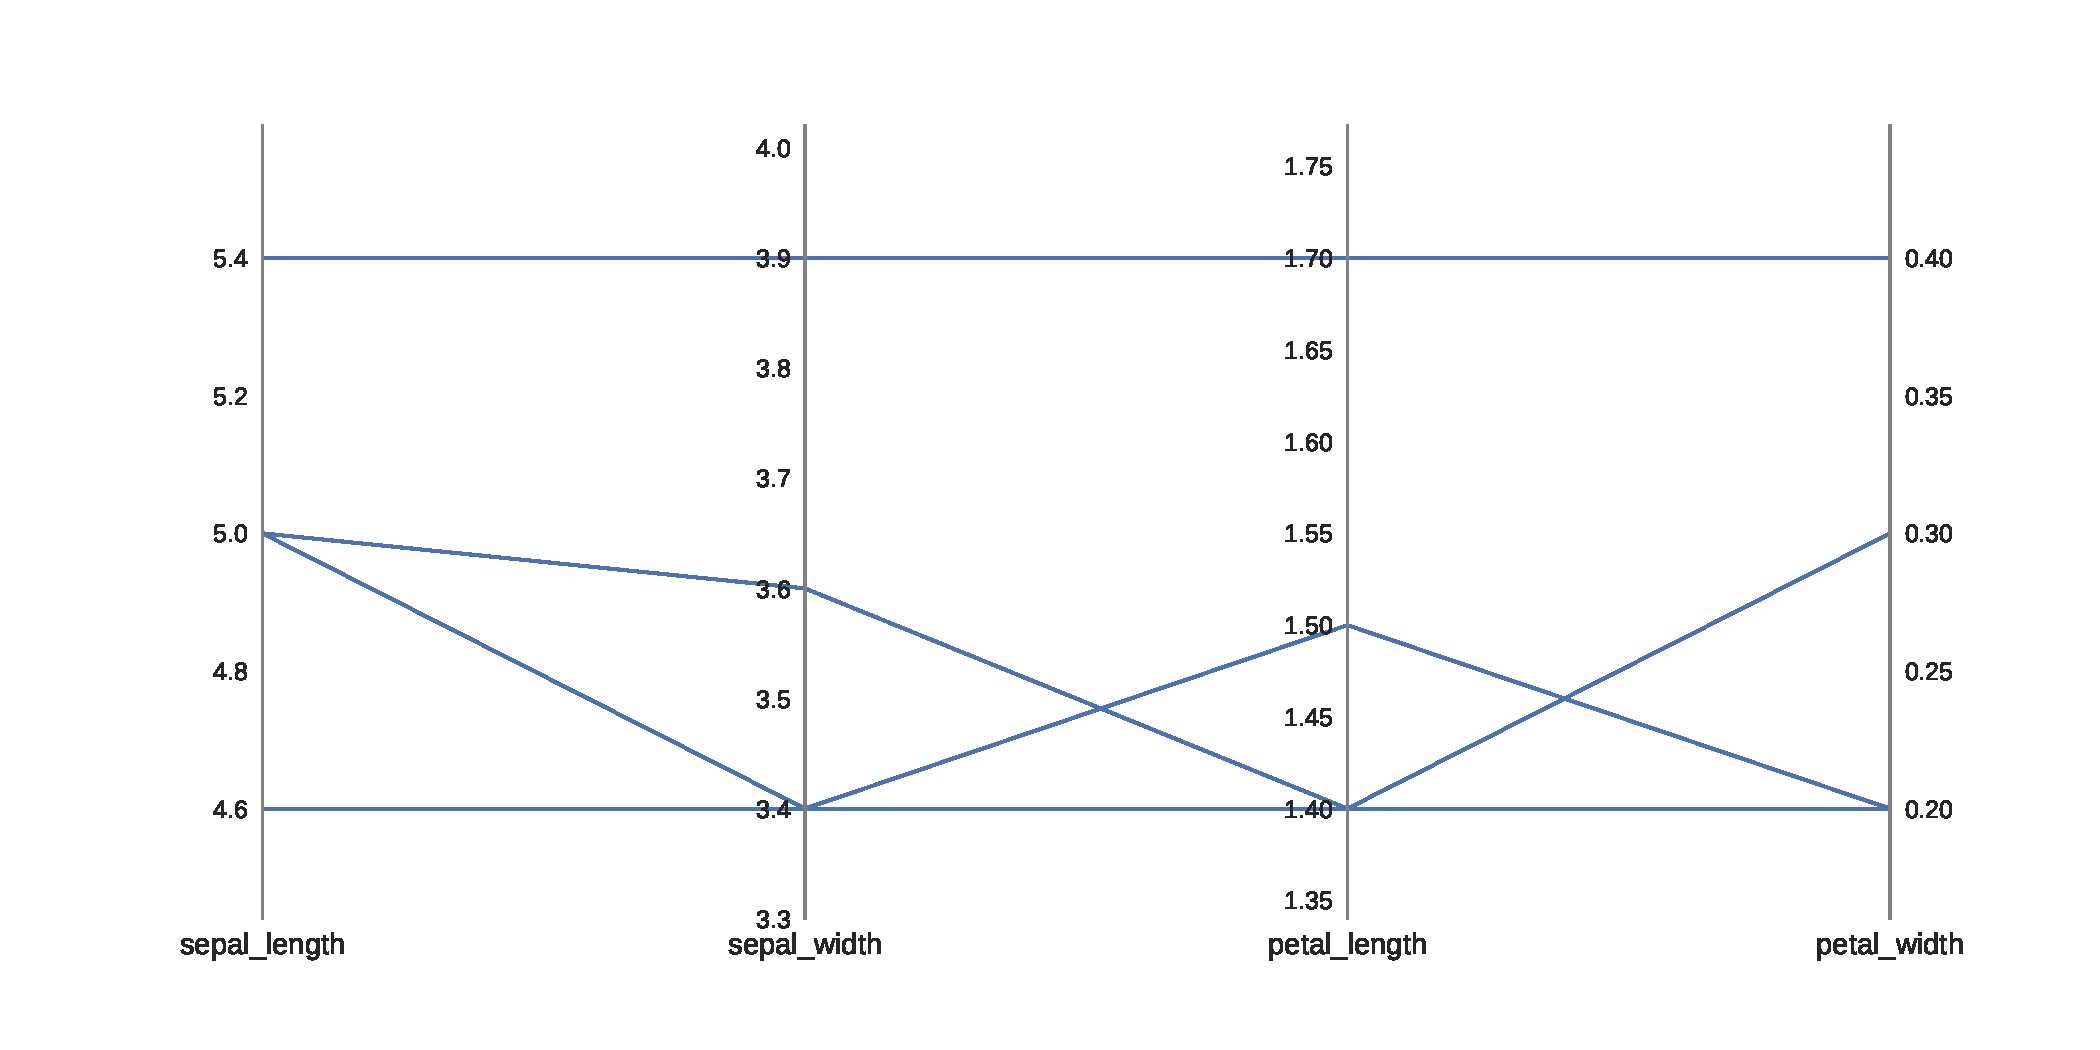
\includegraphics[width=15cm]{classic_pc.pdf}
    \caption{Классический график в параллельных осях}
    \label{classic_pc}
\end{figure}

График в параллельных осях --- метод визуализации многомерных данных.
Для отображения векторов в n-мерном пространстве рисуется n параллельных линий (осей) на одинаковом
расстоянии друг от друга. 
Вектор представляется в виде ломаной кривой, с вершинами на параллельных осях. Точка пересечения
кривой с i-ой осью соответствует i-ой координате объекта.\cite{inselberg_1985}

\noindentВозникают естественные вопросы:
\begin{itemize}
    \item В каком порядке расположить оси?
    \item В какую сторону направлять ось?
    \item Какой масштаб выбрать для каждой оси?
\end{itemize}

\subsection{Модификации}
\subsubsection{1. Добавление кластеров}

\begin{figure}[htb]
    \centering
    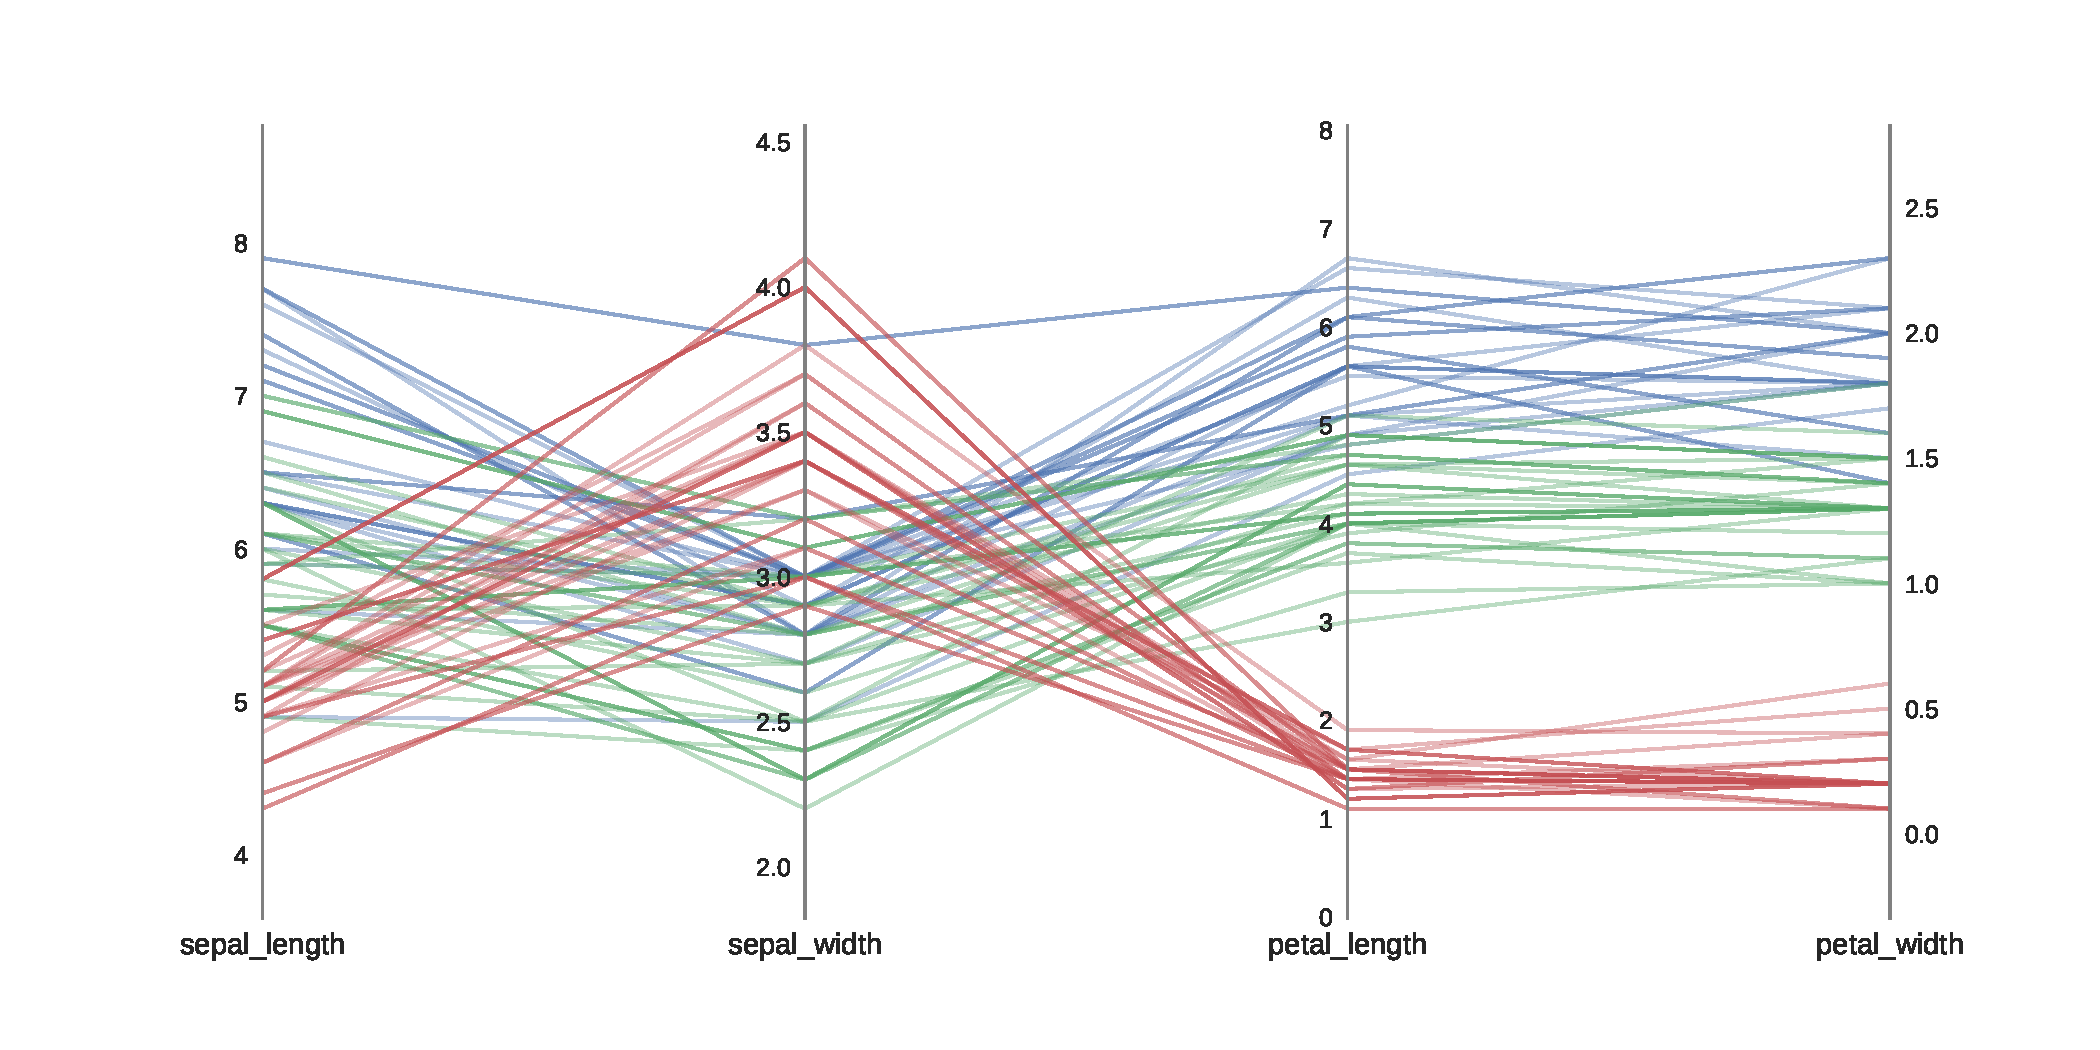
\includegraphics[width=15cm]{color_pc.pdf}
    \caption{График в параллельных осях с кластерами}
    \label{color_pc}
\end{figure}

К сожалению, классический график в параллельных осях становится практически нечитаемым при увеличении 
количества объектов и осей, поэтому чаще всего его применяют в модифицированном виде ---
каждому объекту из выборки ставят в соответствие некоторую категориальную метку по какому-то правилу\footnote{
Обычно правило выбирают так, чтобы объекты с одной меткой были ''похожими'' в некотором смысле --
это называют кластеризацией. Иногда правило может естественным образом вытекать из самих данных,
например, различные виды растений.},
а далее линия, соответствующая объекту, окрашивается в некоторый цвет однозначный метке объекта.
Таким образом на графике можно проследить как ведут себя ''похожие'' объекты.

Но многие проблемы от этого не исчезают:
\begin{itemize}
    \item По прежнему теряется читаемость при увеличении количества объектов и признаков.
    \item Ломанные линии воспринимаются человеком сложнее.
    \item Какое правило выбрать для разметки объектов?
\end{itemize}

\subsubsection{2. Гладкость линий}

\begin{figure}[htb]
    \centering
    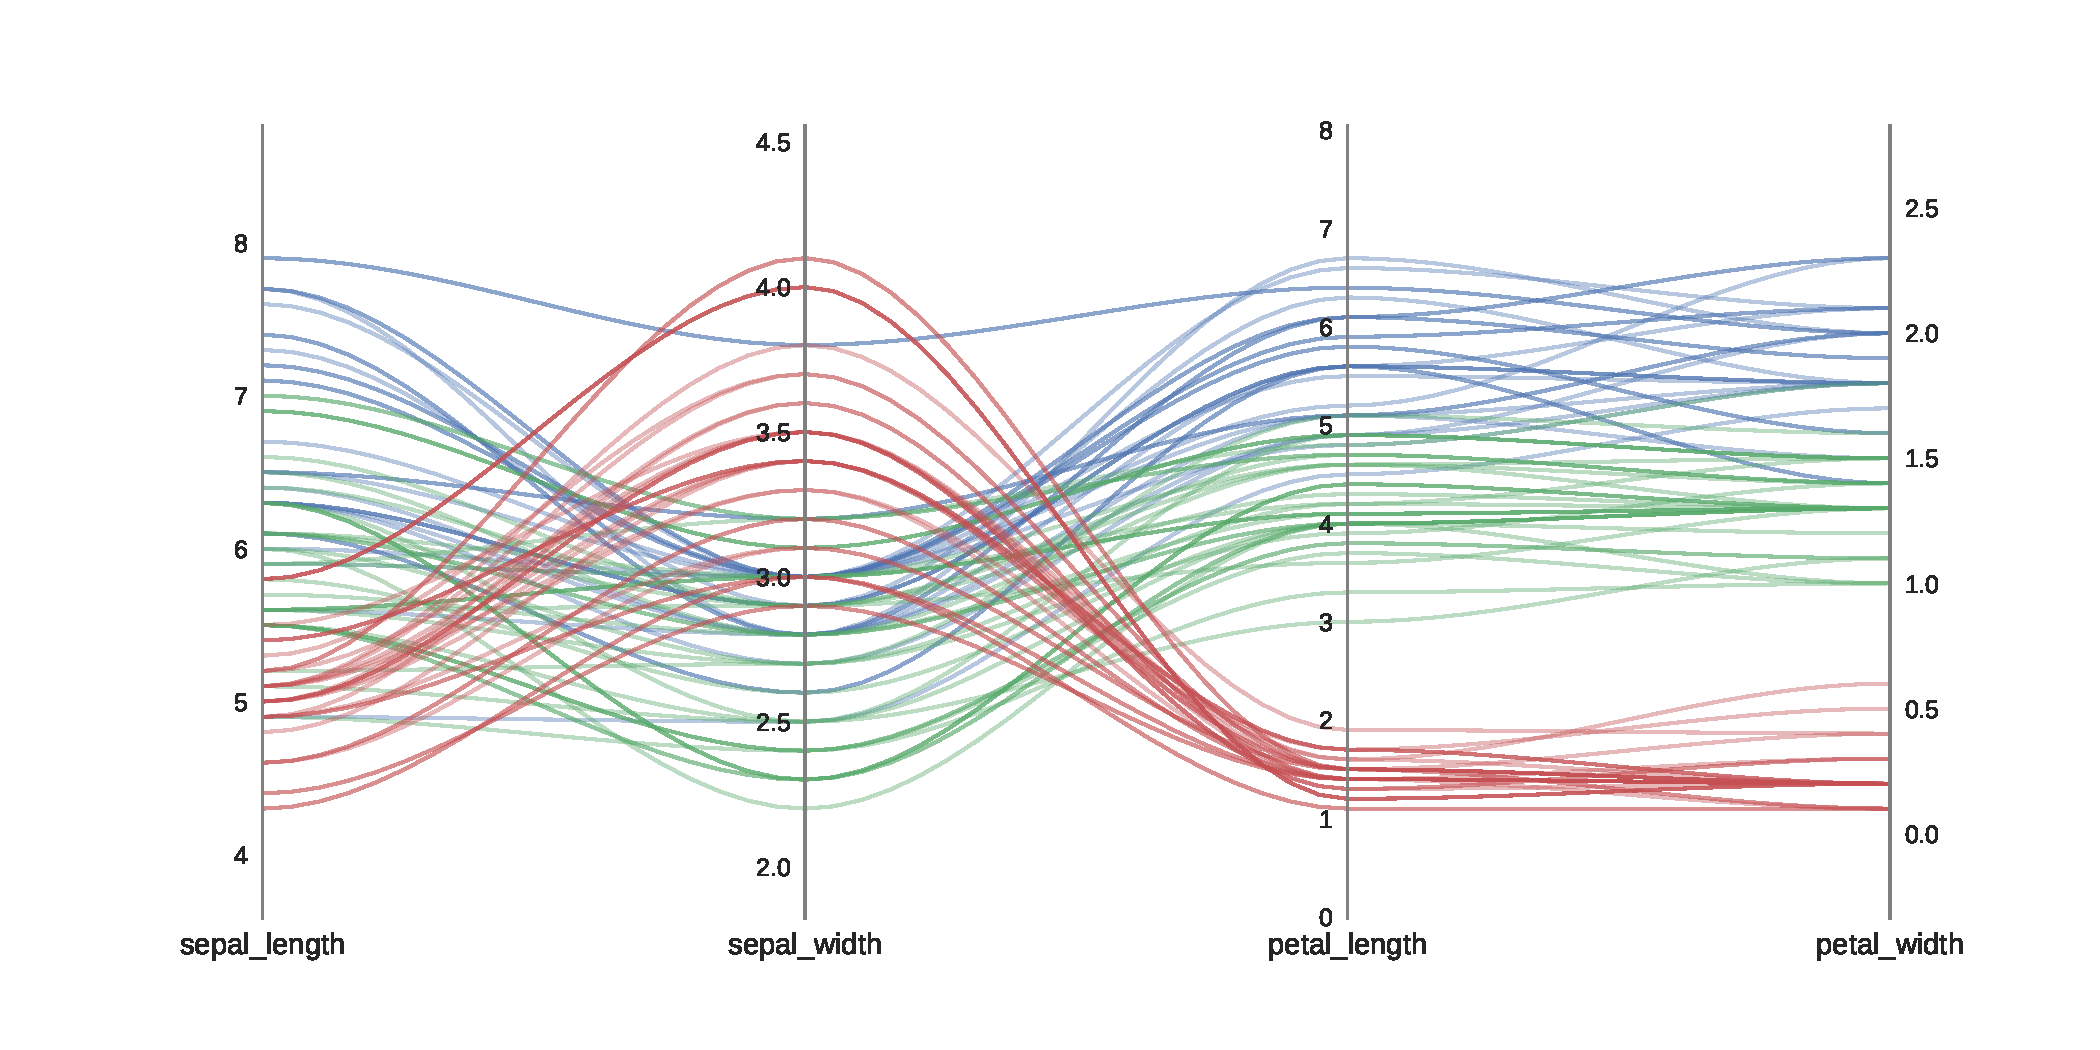
\includegraphics[width=15cm]{smooth_pc.pdf}
    \caption{График в параллельных осях с гладкими линиями}
    \label{smooth_pc}
\end{figure}

Нет никакой необходимости рисовать именно ломанные линии, можно рисовать гладкие кривые, 
которые ''входят'' под некоторым углом к оси (чаще всего перпендикулярно).
Человеку легче воспринимать гладкие линии, поэтому
читаемость графика существенно возрастает.\cite{state_of_the_art}

\subsubsection{3. Связывание линий}

\begin{figure}[htb]
    \centering
    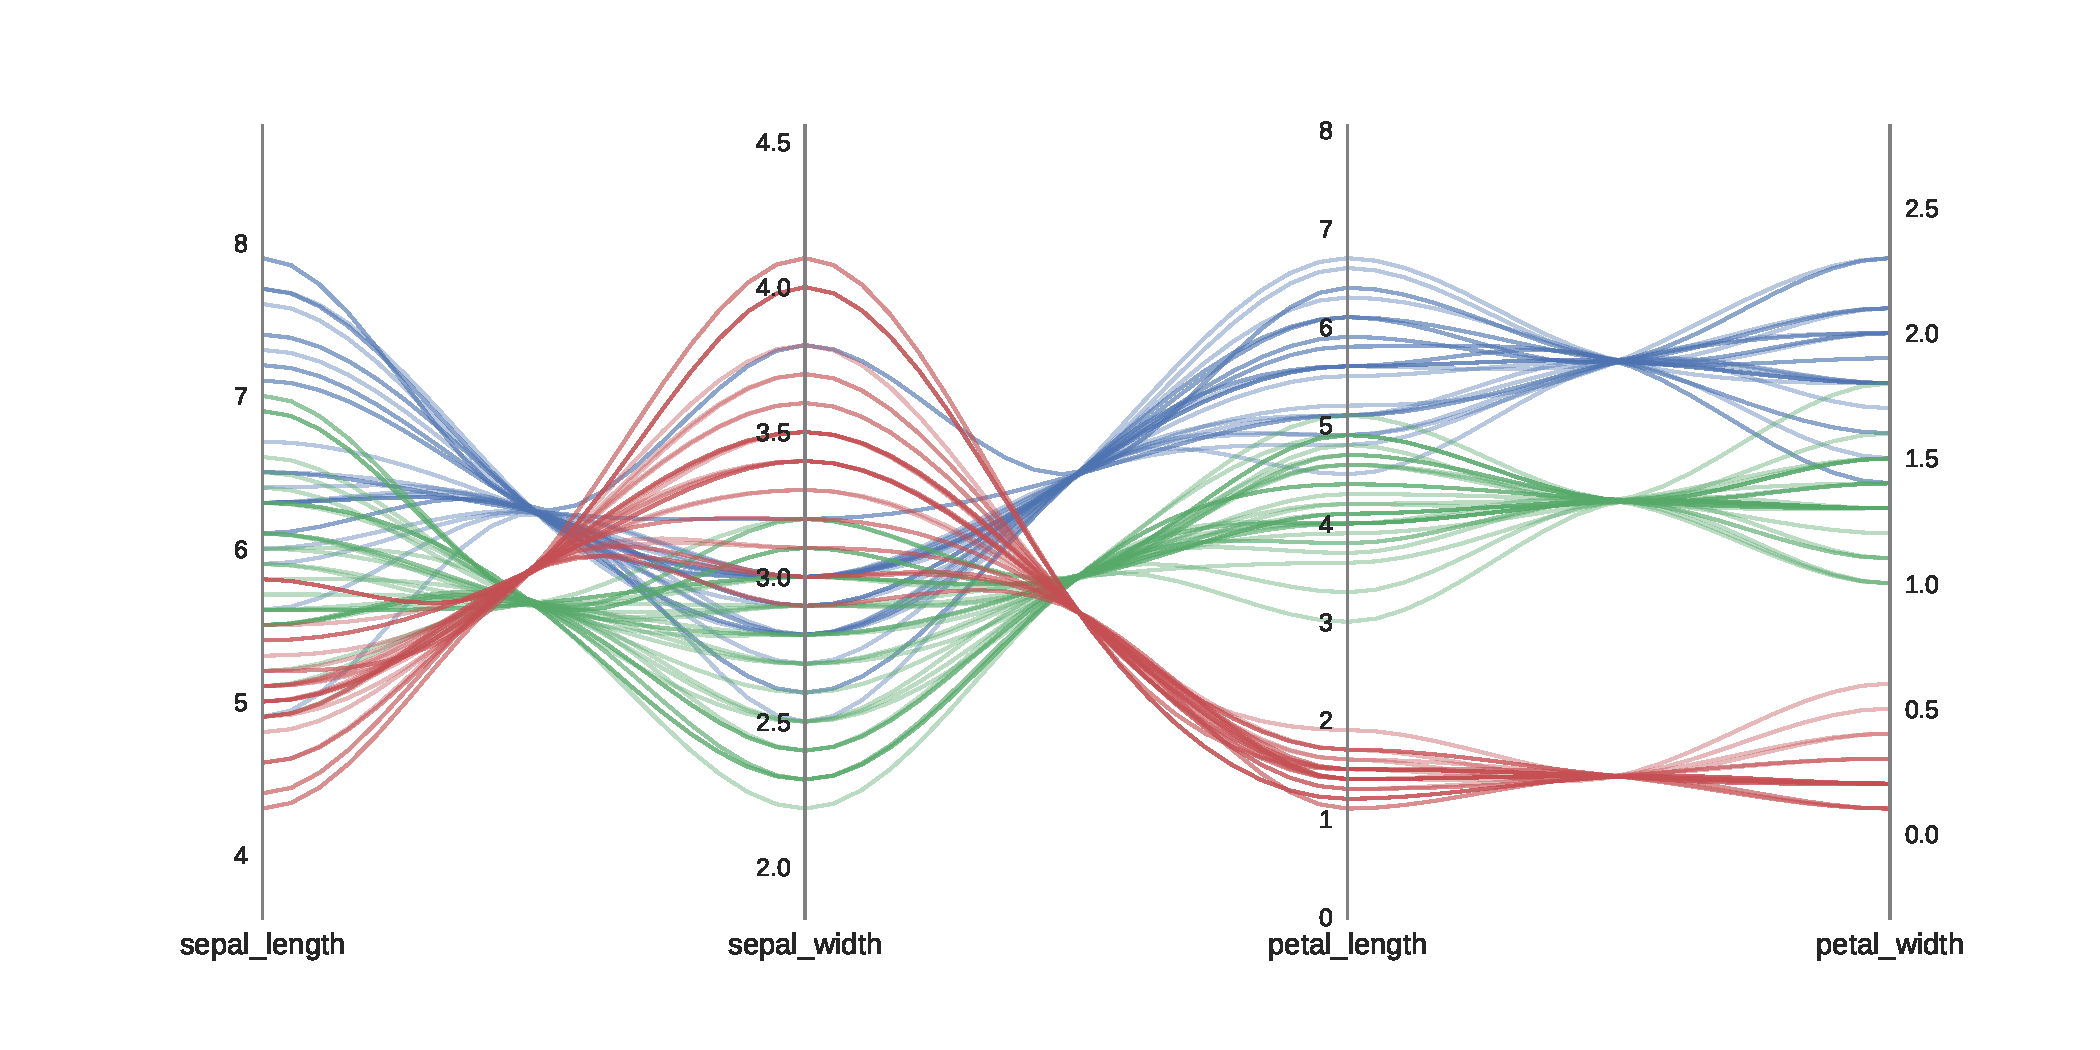
\includegraphics[width=15cm]{bundle_0.01_pc.pdf}
    \caption{График в параллельных осях со ''жгутами''}
    \label{bundle0.01_pc}
\end{figure}

Линии с одинаковыми метками могут связываться в ''жгут'' между парой осей, а 
далее распадаться к соответствующим точкам на оси. Степень связанности регулируема.\cite{bundling}

Эту идею можно обобщить -- пусть линии связываются не потому что принадлежат одному классу, 
а потому что имеют близкие значения координат i и i+1 при построении. Потенциально это избавляет
от необходимости кластеризовать объекты перед построением.

\subsubsection{4. Иерархические графики в параллельных осях}
\begin{figure}[htb]
    \centering
    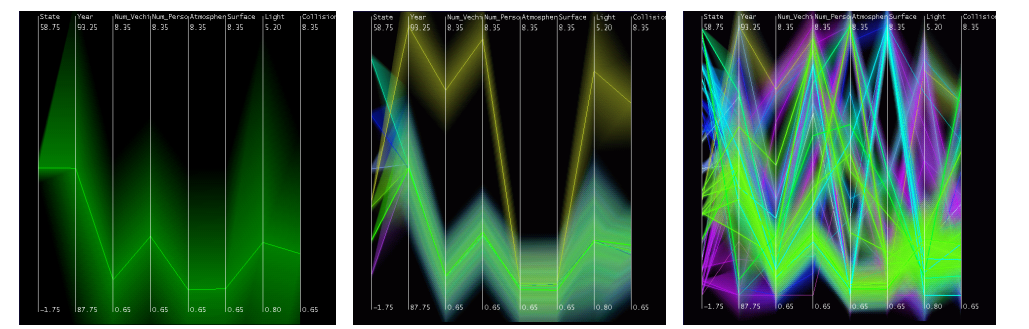
\includegraphics[width=14cm]{hierarchical.png}
    \caption{Иерархические графики начиная с корня и заканчивая большим количеством кластеров}
    \label{hierarchical_coords}
\end{figure}
Иерархические графики в параллельных осях представляют собой метод визуализации не объектов, а иерархических
кластерных структур --- дендрограмм. Вместо визуализации конкретных объектов будем
визуализировать сообщества похожих объектов. Чтобы визуализировать сообщества (кластеры)
нужно выбрать некоторые статистики, например среднее или стандартное отклонение. Среднее нарисуем обычной линией, а 
стандартное отклонение отобразим полупрозрачным градиентом (Рис.\ref{hierarchical_coords}).
Так график становится более читабельным, а детализация регулируется с
помощью включения новых кластеров из дендрограммы.\cite{hierarchical}

\section{Библиотека визуализации}
\subsection{Обзор текущих прикладных средств}
Несмотря на то, что написано большое количество работ о графиках в параллельных осях, 
существует лишь несколько программ, общедоступных для работы с ними.
Например: ELKI, GGobi, Mondrian, Orange и ROOT. Отдельно выделяется D3.Parcoords.js -- 
мощная библиотека на языке JavaScript, посвященная только графикам в параллельных осях.
В python в библиотеке pandas есть лишь его базовая версия. В других же популярных
python библиотеках нет даже этого.

Удивительно, что такое мощное средство визуализации обходят стороной разработчики библиотек. 
Возникает желание создать собственный продукт со всеми возможными подходами к рисованию графика 
в параллельных осях.
\subsection{Цели и задачи библиотеки}
В первую очередь необходимо заметить, что библиотека пишется на базе 
matplotlib. Это очень мощная низкоуровневая библиотека, умеющая рисовать всевозможные 
статические диаграммы. Статичность диаграммы можно считать как недостатком, так и достоинством\footnote{
    В сфере визуализации монополия на использование интерактивных графиков отдана JavaScript и
его библиотекам. Статичные графики обычно рисуют с помощью matplotilb или библиотек, созданных на его базе.}. 
С одной стороны интерактивность в случае графиков в параллельных осях существенно ускоряет построение
эстетичного графика, но с другой это может излишне перегружать и усложнять взаимодействие
пользователя с библиотекой, а также существенно уменьшить спектр возможностей. Библиотека на базе 
matplotilb позволит пользователю не только тончайшим образом настраивать вид графика, но и быстро
получить красивый и информативный график ''из коробки''.
\footnote{Примером может служить библиотека seaborn, написанная на базе matplotlib, но
использующая высокоуровневые функции, позволяющие избегать утомляющей настройки.}

\subsubsection{Возможности библиотеки:}
\begin{itemize}
    \item Построение классических графиков в параллельных осях
    \begin{itemize}
        \item Возможность рисовать гладкие линии. Должен быть непрерывный параметр,
        задаюший вид кривой.
        \item Возможность ''связывания'' линий кластеров.
        Должен быть непрерывный параметр задающий степень связывания.
        \item Возможность ''связывания'' линий на основе близости. Также 
        должен быть непрерывный параметр задающий степень связывания. 
    \end{itemize}
    \item Построение иерархических графиков
    \begin{itemize}
        \item Отрисовка полупрозрачного градиента.
        \item Работа с иерархическими кластерами(дендрограммами).
        \item Изображение распределения с помощью градиента (boxplot, histogram).
    \end{itemize}
    \item Дополнительно
    \begin{itemize}
        \item выделение подмножества линий в  диапазоне значений одной из осей.
        \item нахождение оптимального расположения осей.
        \item создание иерархических кластеров на основе входящей выборки.
    \end{itemize}
\end{itemize}

\subsubsection{Технические особенности:}
\begin{itemize}
    \item Простой высокоуровневый интерфейс. Как и в библиотеке seaborn методы могут принимать pandas.DataFrame,
    обычные numpy массивы или списки -- для всего единый интерфейс.
    \item Эстетичные графики ''из коробки''.
\end{itemize}

\subsection{Итоги(после первого семестра)}
По итогам семестра удалось реализовать большую часть возможностей библиотеки, касающихся классического
графика в параллельных осях
\begin{itemize}
    \item Возможность рисовать гладкие линии. \textbf{Пока что не добавлен параметр задающий вид кривой}.
    \item Возможность ''связывания'' линий кластеров. 
    Добавлен непрерывный параметр задающий степень связывания.
    \item \textbf{Возможность связывания линий на основе близости не реализована}
\end{itemize}

Интерфейс для пользователя практически полностью повторяет реализацию seaborn. Пока что в качестве 
параметра доступен только pandas.DataFrame, но уже сейчас можно получать красивые графики ''из коробки''.\footnote{
    Большинство графиков в отчете нарисованы с помощью данной библиотеки.}

\begin{thebibliography}{99}
    \bibitem{inselberg_1985} Inselberg A., Dimsdale B. Parallel coordinates: 
    a tool for visualizing multi-dimensional geometry 
    //Proceedings of the First IEEE Conference on Visualization: 
    Visualization90. – IEEE, 1990. – С. 361-378.
    \bibitem{state_of_the_art} Heinrich J., Weiskopf D. State of the Art of Parallel Coordinates 
    //Eurographics (STARs). – 2013. – С. 95-116.
    \bibitem{bundling} Heinrich J. et al. Evaluation of a bundling technique for parallel coordinates 
    //arXiv preprint arXiv:1109.6073. – 2011.
    \bibitem{hierarchical} Fua Y. H., Ward M. O., Rundensteiner E. A. Hierarchical parallel coordinates
     for exploration of large datasets. – IEEE, 1999. – С. 43-508.
\end{thebibliography}
\end{document}